
\section{Effectiveness}

\subsection{Definitions}

A navigation is defined as
a search, or
a click on an instructor’s name, or
a click on a crosslisted or prerequisite course link

The navigations-per-add measure is
the number of navigations a user took (within one session) until a course was added, bookmarked

\subsection{Trends}

\begin{figure}[H]
  \centering
  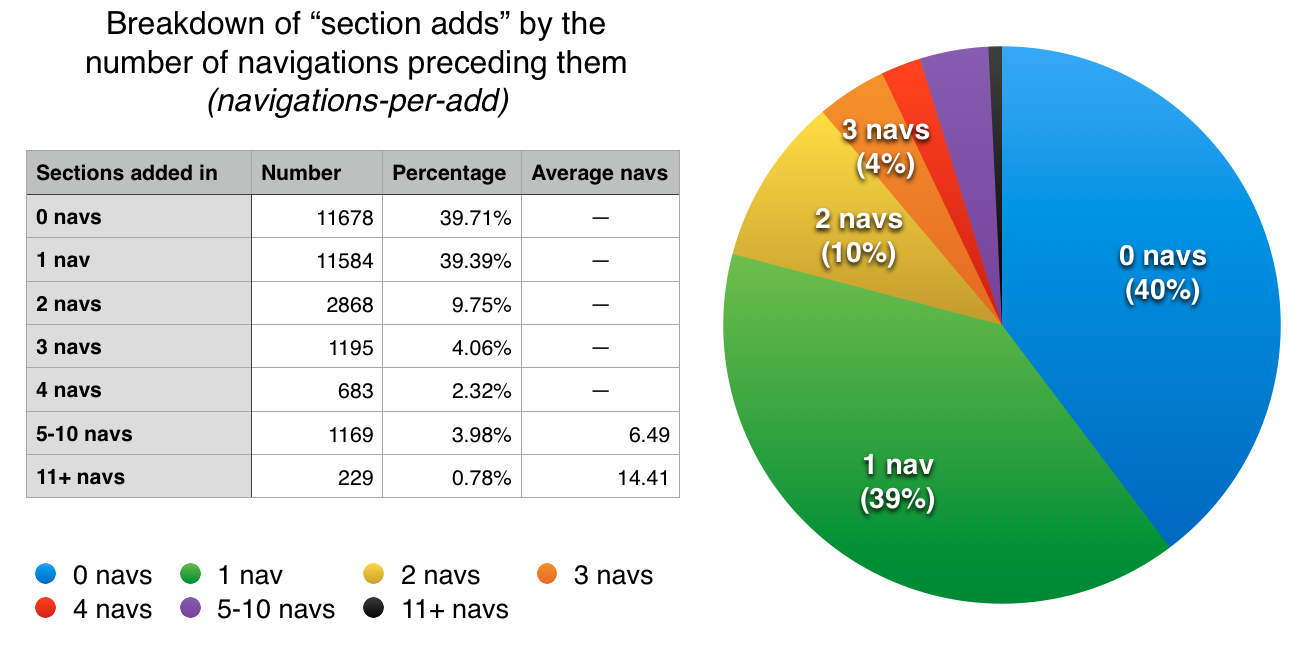
\includegraphics[width=1.0\textwidth]{images/graph/combined_navs}

  \caption{Etc}
  \label{fig:searchtypes}
\end{figure}

\subsection{Breaking them apart}

  behavioral patterns
  Direct search for specific course
  Discovery, browsing, exploring

  \subsubsection{Direct searches}

  \begin{figure}
    \centering
    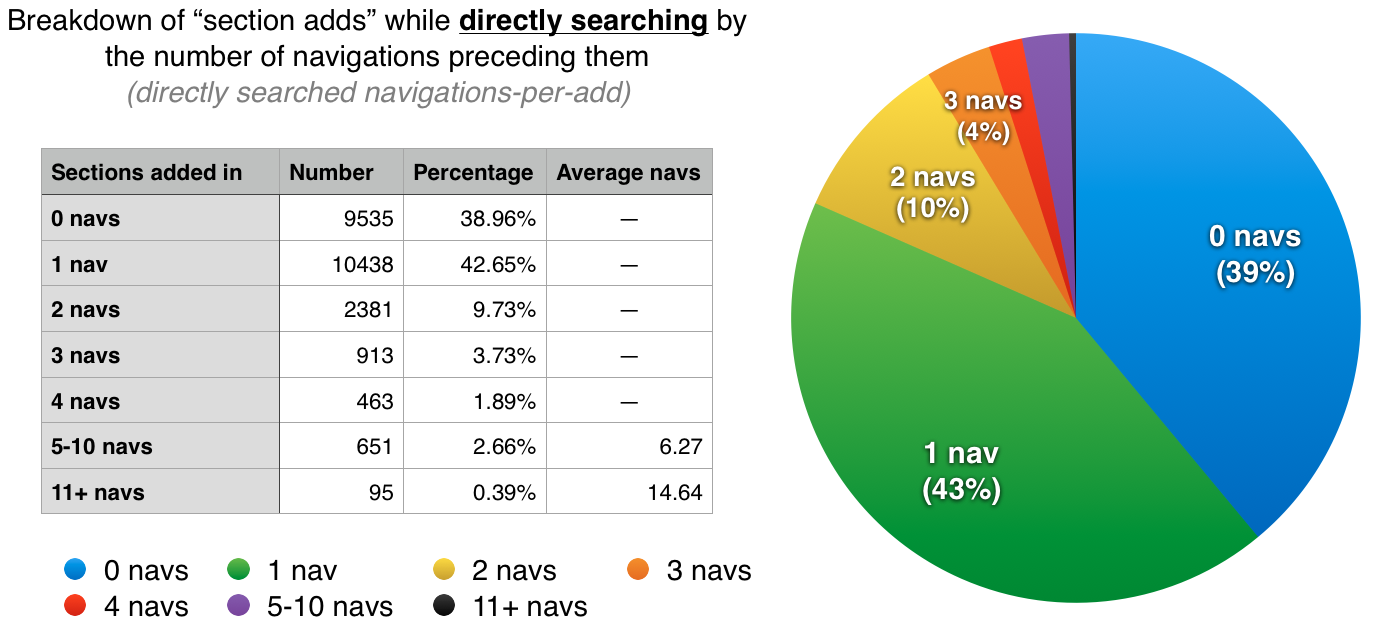
\includegraphics[width=1.0\textwidth]{images/graph/direct_navs}

    \caption{Etc}
    \label{fig:searchtypes}
  \end{figure}

  Why would 0-navs be so common with direct searches? 64\% of them subsections!

  \subsubsection{Browse}

  \begin{figure}
    \centering
    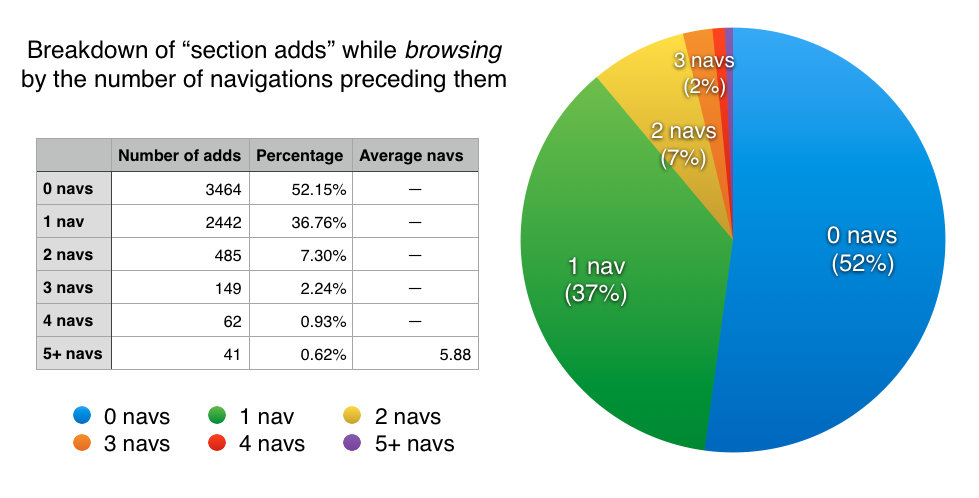
\includegraphics[width=1.0\textwidth]{images/graph/browse_navs}

    \caption{Etc}
    \label{fig:searchtypes}
  \end{figure}

  As expected, the 0-navs were mostly maincourses (62\%)

  Effective++

  \subsubsection{Social}

  90 users have linked Skedge to Facebook
  Since March 1st,
  4,000+ visits (200 visits/day)
  ~60\% of visits to /social were returning visitors
  90 overlays onto friends’ schedules
  10 clicks to Facebook profiles :(
  - get stats from the fb dashboard

  success?????